% MIT License
%
% Ankit Maurya
% ankit.dp@bhu.ac.in
%
% Permission is hereby granted, free of charge, to any person obtaining a copy
% of this software and associated documentation files (the "Software"), to deal
% in the Software without restriction, including without limitation the rights
% to use, copy, modify, merge, publish, distribute, sublicense, and/or sell
% copies of the Software, and to permit persons to whom the Software is
% furnished to do so, subject to the following conditions:
%
% The above copyright notice and this permission notice shall be included in all
% copies or substantial portions of the Software.
%
% THE SOFTWARE IS PROVIDED "AS IS", WITHOUT WARRANTY OF ANY KIND, EXPRESS OR
% IMPLIED, INCLUDING BUT NOT LIMITED TO THE WARRANTIES OF MERCHANTABILITY,
% FITNESS FOR A PARTICULAR PURPOSE AND NONINFRINGEMENT. IN NO EVENT SHALL THE
% AUTHORS OR COPYRIGHT HOLDERS BE LIABLE FOR ANY CLAIM, DAMAGES OR OTHER
% LIABILITY, WHETHER IN AN ACTION OF CONTRACT, TORT OR OTHERWISE, ARISING FROM,
% OUT OF OR IN CONNECTION WITH THE SOFTWARE OR THE USE OR OTHER DEALINGS IN THE
% SOFTWARE.

\documentclass[12pt,a4paper]{report}

% Packages
\usepackage{geometry}
\usepackage{fancyhdr}
\usepackage{setspace}
\usepackage{titlesec}
\usepackage{graphicx}
\usepackage{caption}
\usepackage{amsmath,amssymb}
\usepackage{booktabs}
\usepackage{array}
\usepackage{tabularx}
\usepackage{xcolor}
\usepackage{listings}
\usepackage{tikz}
\usepackage[colorlinks=true,linkcolor=black,citecolor=blue!60!black,urlcolor=blue!60!black,linktoc=all]{hyperref}
\usetikzlibrary{positioning,arrows.meta,calc,fit,backgrounds}

% Set page margins
\geometry{top=1in, bottom=1in, left=1in, right=1in}

% Page numbering format
\pagestyle{fancy}
\fancyhf{}
\rfoot{\thepage}
\renewcommand{\headrulewidth}{0pt}

% Chapter and Section formatting
\titleformat{\chapter}[display]
  {\normalfont\fontsize{14}{16}\selectfont\bfseries\centering}{\MakeUppercase{\chaptertitlename}\ \thechapter}{20pt}{\fontsize{14}{16}\selectfont\bfseries}
\titleformat{\section}
  {\normalfont\fontsize{12}{14}\selectfont\bfseries}{\thesection}{1em}{}
\titleformat{\subsection}
  {\normalfont\fontsize{12}{14}\selectfont\bfseries}{\thesubsection}{1em}{}
\titleformat{\subsubsection}
  {\normalfont\fontsize{12}{14}\selectfont\bfseries}{\thesubsubsection}{1em}{}
\titlespacing*{\chapter}{0pt}{-10pt}{22pt}

% Table of Contents formatting
\makeatletter
\renewcommand*\l@chapter[2]{%
  \ifnum \c@tocdepth >\m@ne
    \addpenalty{-\@highpenalty}%
    \vskip 1.0em \@plus\p@
    \setlength\@tempdima{1.5em}%
    \begingroup
      \parindent \z@ \rightskip \@pnumwidth
      \parfillskip -\@pnumwidth
      \leavevmode \bfseries
      \advance\leftskip\@tempdima
      \hskip -\leftskip
      #1\nobreak\hfil \nobreak\hb@xt@\@pnumwidth{\hss #2}\par
      \penalty\@highpenalty
    \endgroup
  \fi}

\renewcommand*\l@section{\@dottedtocline{1}{0em}{2.3em}}
\renewcommand*\l@subsection{\@dottedtocline{2}{2.3em}{3.2em}}
\renewcommand*\l@subsubsection{\@dottedtocline{3}{5.5em}{4.1em}}
\renewcommand*\l@paragraph{\@dottedtocline{4}{8.6em}{5em}}
\renewcommand*\l@subparagraph{\@dottedtocline{5}{12em}{6em}}
\makeatother

% ------------------------------------------------------------------
% Project-specific definitions
% ------------------------------------------------------------------
\definecolor{tealfill}{HTML}{DDF1EE}   \definecolor{tealline}{HTML}{0F766E}
\definecolor{purplefill}{HTML}{E8E1F8} \definecolor{purpleline}{HTML}{6D4AC4}
\definecolor{coralfill}{HTML}{FBE3DF}  \definecolor{coralline}{HTML}{C8472B}
\definecolor{grayfill}{HTML}{EEF1F4}   \definecolor{grayline}{HTML}{64748B}

\tikzset{
  tbox/.style={draw=tealline,   fill=tealfill,   rounded corners=2pt, align=center, font=\small, text width=6.0cm, minimum height=0.95cm, inner sep=3pt},
  pbox/.style={draw=purpleline, fill=purplefill, rounded corners=2pt, align=center, font=\small, text width=6.0cm, minimum height=0.95cm, inner sep=3pt},
  cbox/.style={draw=coralline,  fill=coralfill,  rounded corners=2pt, align=center, font=\small, text width=6.0cm, minimum height=0.95cm, inner sep=3pt},
  gbox/.style={draw=grayline,   fill=grayfill,   rounded corners=2pt, align=center, font=\small, text width=6.0cm, minimum height=0.95cm, inner sep=3pt},
  flow/.style={-{Stealth[length=2.4mm]}, thick, color=grayline}
}

% Highlighted placeholder for values that must be filled in after the experiments are run
\newcommand{\tbd}[1]{\colorbox{yellow}{\textbf{[#1]}}}

% Include a figure if the image file exists, otherwise show a labelled placeholder frame
\newcommand{\maybefigure}[4]{% file, width, height of placeholder, description
  \IfFileExists{figures/#1}{\includegraphics[width=#2]{figures/#1}}{%
    \fbox{\parbox[c][#3][c]{0.92\textwidth}{\centering\textbf{[Insert figure]}\\[2pt] \small #4\\[2pt]
    \footnotesize Save it from the notebook as \texttt{\detokenize{figures/#1}} and recompile.}}}}

% Values produced by make_results_table.py (placeholders until results.csv exists)
\newcommand{\TestDays}{297}
\newcommand{\UpShareTest}{50.2\%}
\newcommand{\BaselineAcc}{50.2\%}
\newcommand{\MarginErr}{$\pm$5.7}
\newcommand{\BestModel}{Logistic Regression}
\newcommand{\BestFeatureSet}{multimodal}
\newcommand{\BestAcc}{49.8\%}
\newcommand{\BestAUC}{0.539}
\newcommand{\NumBestAUC}{0.520}
\newcommand{\MMBestAUC}{0.539}
\newcommand{\AUCDelta}{+0.019}
\newcommand{\TrainDays}{1384}
\newcommand{\ValDays}{297}
\newcommand{\TrainRange}{22 Aug 2008 to 21 Feb 2014}
\newcommand{\ValRange}{24 Feb 2014 to 28 Apr 2015}
\newcommand{\TestRange}{29 Apr 2015 to 30 Jun 2016}


% Code listings
\lstset{
  language=Python, basicstyle=\ttfamily\footnotesize, keywordstyle=\bfseries, commentstyle=\itshape\color{grayline},
  stringstyle=\color{coralline}, breaklines=true, frame=single, framerule=0.3pt, rulecolor=\color{grayline},
  backgroundcolor=\color{grayfill!60}, xleftmargin=2pt, xrightmargin=2pt, aboveskip=8pt, belowskip=4pt,
  columns=fullflexible, keepspaces=true, showstringspaces=false
}
\captionsetup{font=small, labelfont=bf, skip=6pt}
% let floats fill pages instead of leaving white space
\renewcommand{\topfraction}{0.95}\renewcommand{\bottomfraction}{0.95}
\renewcommand{\textfraction}{0.05}\renewcommand{\floatpagefraction}{0.8}
\setcounter{topnumber}{3}\setcounter{bottomnumber}{3}\setcounter{totalnumber}{5}
\raggedbottom

% Title Page
\begin{document}
\begin{titlepage}
    \centering

    % Title
    {\Huge \bfseries{Stock Trend Prediction using Machine Learning}\par}
    \vspace{1cm}
    {\large A report submitted in partial fulfillment of the requirements for\par}
    {\large\itshape the subject of Machine Learning\par}
    \vspace{1cm}
    {\Large\bfseries B.Tech in Computer Science and Engineering\par}  % Uncomment this for MCA
    % {\Large\bfseries Master of Science\par}   % Uncomment this for M.sc
    \vspace{1cm}
    {\large by\par}
    \vspace{1cm}
    {\Large\bfseries Kundan Kumar (SIC-24BCSG85, Roll-6)\par}
    \vspace{0.2cm}
    {\Large\bfseries Soham Mohanty (SIC-24BCSD49, Roll-3)\par}
    \vspace{0.2cm}
    {\Large\bfseries Priyanshu Sekhar Badhei (SIC-24BCSF35, Roll-4)\par}
    \vspace{0.2cm}
    {\Large\bfseries Naman Verma (SIC-24BCSF15, Roll-2)\par}
    \vspace{0.2cm}
    {\Large\bfseries Tejash Arya (SIC-24BCSG63, Roll-15)\par}
    \vspace{1cm}
    % University Logo
    
\includegraphics[width=0.4\textwidth]{silicon_university_logo.png}\\
    \vspace{1cm}
    % Department and University
    {\Large\bfseries Department of Computer Science and Engineering\par}

    {\Large\bfseries Silicon University  - 751024\par}

\end{titlepage}

% Preliminaries

% Abstract
\chapter*{Abstract}
\addcontentsline{toc}{chapter}{Abstract}
\begin{spacing}{1.2}
Predicting short-term stock market movements is a challenging task due to the complex,
volatile, and highly dynamic nature of financial markets. Traditional prediction approaches often
rely primarily on historical market data and technical indicators, while ignoring the influence of
financial news and investor sentiment. On the other hand, sentiment-based approaches may
overlook important numerical patterns present in market data. This project proposes a
multimodal machine learning framework that combines these two sources of information to
predict the next-day direction of the S\&P 500 Index.
\newline
The proposed system uses historical S\&P 500 market data obtained through financial data
sources and extracts numerical features such as returns, Relative Strength Index (RSI), Moving
Average Convergence Divergence (MACD), and trading volume. In parallel, financial news
headlines are processed using FinBERT, a transformer-based language model specialized for
financial text, to obtain positive, negative, and neutral sentiment scores. The two modalities are
then aligned chronologically and combined into a unified feature set while maintaining a strict
time-based data split to reduce the risk of data leakage and look-ahead bias.
\newline
The fused dataset is used to train and compare multiple supervised machine learning
models, including Logistic Regression, XGBoost, and Random Forest, for binary classification
of the next trading day's market direction as Up or Down. Model performance is evaluated
using accuracy, precision, recall, F1-score, ROC-AUC, and confusion matrices. The study
also compares numerical-only, sentiment-only, and multimodal approaches to examine whether
combining financial news sentiment with technical market information provides additional
predictive value.
\newline
On a held-out test period of 297 trading days, test accuracy of the nine model and feature-set
combinations ranged from 47.8\% to 52.2\% against a majority-class baseline of 50.2\%, and
ROC-AUC from 0.481 to 0.539. The multimodal model improved the best numerical-only ROC-AUC
by only 0.019, which is within sampling error, so no model showed predictive skill beyond
chance. Most models predicted the Up class on the great majority of days, and their balanced
accuracy was about 0.50. The result is consistent with the efficient market hypothesis. A demonstration
forecast for the next trading day, made with technical indicators only because no live news feed is
available, is included to show how the pipeline is applied to current data.
\newline
The project aims to demonstrate a practical application of Natural Language Processing
and machine learning in financial forecasting while providing an interpretable and reproducible
framework suitable for academic experimentation.
\end{spacing}
\clearpage

% Candidate's Declaration
\chapter*{Candidate's Declaration}
\addcontentsline{toc}{chapter}{Candidate's Declaration}
\begin{spacing}{1.2}
I hereby certify that the work, which is being presented in the project report, entitled \textbf{Stock Trend Prediction using Machine Learning}, in partial fulfillment of the requirement for the award of the B.Tech in Computer Science and Engineering  and submitted to the institution is an authentic record of my own work carried out during the period \textbf{start  to end} under the supervision of \textbf{Dr. Pradipta Kumar Pattanayak}.

I also cited the reference about the text(s)/figure(s)/table(s)/equation(s) from where they have been taken.
\newline

The matter presented in this report has not been submitted elsewhere for the award of any other degree or diploma from any institutions.
\newline
\newline
\newline

\textbf{Date:} \rule{3cm}{.15mm} \hspace{5cm} \textbf{Signature of the Candidate }
\newline
\rule{0cm}{0mm} \hspace{9cm} \textbf{1.}
\newline
\newline
\rule{0cm}{0mm} \hspace{9cm} \textbf{2.}
\newline
\newline
\rule{0cm}{0mm} \hspace{9cm} \textbf{3.}
\newline
\newline
\rule{0cm}{0mm} \hspace{9cm} \textbf{4.}
\newline
\newline
\rule{0cm}{0mm} \hspace{9cm} \textbf{5.}


\vspace{1cm}

This is to certify that the above statement made by the candidate is correct to the best of my knowledge.

\vspace{3cm}

\begin{minipage}[t]{0.3\textwidth}
\begin{center}

    \textbf{Signature of \\ Supervisor(s)} \\

    \end{center}
\end{minipage}%
\hfill
\begin{minipage}[t]{0.4\textwidth}
\begin{center}



    \end{center}
\end{minipage}
\end{spacing}
\clearpage

% Acknowledgements
\chapter*{Acknowledgements}
\addcontentsline{toc}{chapter}{Acknowledgements}

We would like to express our sincere gratitude to our project guide, Dr.\ Pradipta Kumar Pattanayak, for his invaluable guidance, constructive feedback, and continuous encouragement throughout the course of this project. His insights into machine learning methodology and time-series evaluation practices were instrumental in shaping the direction and rigor of this work.

We are also thankful to the faculty of the Department of Computer Science and Engineering for providing the academic environment and resources necessary to carry out this work, and to our peers for the many helpful discussions that clarified our understanding of the underlying concepts.

Finally, we would like to thank our families and friends for their unwavering support and patience during the course of this project.

\clearpage

% Table of Contents, List of Figures and List of Tables
\tableofcontents
\clearpage
\listoffigures
\clearpage
\listoftables
\clearpage

% Main content
\chapter{Introduction}

\section{Background and Motivation}
Financial markets aggregate the beliefs, expectations and decisions of millions of participants, and the prices they produce change every second. For individual investors, institutions and researchers alike, the ability to anticipate even the direction of the next day's move in a broad index would be valuable. The S\&P 500 index, which tracks the share prices of 500 large companies listed on United States exchanges, is the most widely followed benchmark of the American equity market and is therefore a natural target for such an effort.

Two families of information are traditionally used to reason about short-term price movements. The first is \emph{numerical market data}: the history of prices and traded volume, and the technical indicators derived from them, such as returns, the Relative Strength Index (RSI) and the Moving Average Convergence Divergence (MACD). The second is \emph{textual information}: news headlines, reports and social media posts through which new information reaches investors and shapes their mood. Most published machine learning studies use only one of the two. Price-based models ignore the context in which the prices were formed, and text-based models ignore the numerical regime (trending, oversold, high-volume) that determines how the market reacts to a given piece of news.

Recent advances in Natural Language Processing (NLP) make it practical to combine both. Transformer language models such as BERT~\cite{devlin2019bert} can be fine-tuned for specialised domains, and FinBERT~\cite{araci2019finbert} is one such model trained on financial text. It converts a headline into probabilities of positive, negative and neutral sentiment, which are numbers that a conventional classifier can consume alongside technical indicators. This opens the door to a \emph{multimodal} approach, in which two different modalities (numbers and text) are fused into a single model.

\section{Problem Statement}
The problem addressed in this project is stated as follows.

\begin{quote}
\emph{Given the market data and the news headlines available up to the close of trading day $t$, predict whether the closing value of the S\&P 500 index on day $t+1$ will be higher (Up) or lower or equal (Down) than its closing value on day $t$.}
\end{quote}

This is a supervised binary classification problem. Let $x_t$ denote the feature vector assembled from information available at the end of day $t$, and let
\begin{equation}
y_t =
\begin{cases}
1 & \text{if } P_{t+1} > P_t,\\
0 & \text{otherwise,}
\end{cases}
\label{eq:target}
\end{equation}
where $P_t$ is the closing value of the index on day $t$. The learning task is to estimate a function $f$ such that $f(x_t) \approx y_t$, with $f$ trained only on days earlier than those on which it is evaluated.

The problem is deliberately difficult. According to the efficient market hypothesis~\cite{fama1970efficient}, prices already reflect all available information, which implies that little or nothing can be gained by modelling past prices and public news. Empirically, next-day direction behaves close to a fair coin: the share of Up days in a bull market is typically only a few percentage points above one half. A credible study of this problem must therefore state its baselines honestly, report uncertainty, and guard against the evaluation mistakes (especially look-ahead bias) that produce spuriously impressive accuracy figures.

\section{Objectives}
The objectives of the project are the following.
\begin{enumerate}
  \item To collect and clean daily S\&P 500 market data and derive numerical features: one-day and five-day returns, RSI, MACD (line, signal and histogram) and the relative change in trading volume.
  \item To score daily financial news headlines with FinBERT and aggregate the scores into daily positive, negative and neutral sentiment features.
  \item To align the two modalities chronologically and fuse them into one feature set without leaking future information into the past.
  \item To train and tune three supervised classifiers, namely Logistic Regression, Random Forest and XGBoost, on the fused features.
  \item To evaluate all models on a strictly later, untouched test period using accuracy, precision, recall, F1-score, ROC-AUC and confusion matrices, and to compare them with a majority-class baseline.
  \item To run an ablation comparing three feature sets (numerical-only, sentiment-only and multimodal) in order to determine whether sentiment adds predictive value beyond technical indicators.
\end{enumerate}

\section{Scope and Assumptions}
The study is limited to the daily frequency and to a single index. The text modality is represented by headlines only, not full articles. The target is the direction of the next close, and no trading strategy, transaction costs or position sizing are modelled; the project therefore makes no claim about profitability. The experiments use a historical window for which a labelled headline corpus is openly available (August 2008 to July 2016), and a live-news extension is described as future work. The work is an academic exercise in applying machine learning and NLP to financial data, and nothing in this report should be construed as investment advice.

\section{Contributions}
The principal contributions of this project are:
\begin{itemize}
  \item a reproducible, notebook-based pipeline that takes the project from raw data download to a final comparison of models;
  \item a leakage-aware design: the sentiment features are shifted by one trading day after the join, the split is chronological, the scaler is fitted on the training data only, and hyper-parameters are tuned with walk-forward cross-validation;
  \item a three-way ablation (numerical, sentiment, multimodal) evaluated with several metrics rather than accuracy alone, together with a majority-class baseline and an estimate of the sampling error of the test accuracy;
  \item a critical review of existing work in this area, identifying the evaluation weaknesses that the present design is intended to avoid.
\end{itemize}

\section{Organisation of the Report}
The remainder of this report is organised as follows. Chapter~2 reviews existing work on news-based and hybrid stock prediction and identifies gaps. Chapter~3 gives the theoretical background on technical indicators, FinBERT, the classifiers and the evaluation metrics. Chapter~4 presents the proposed multimodal approach and its leakage-control design. Chapter~5 describes the implementation, including the data sources, the feature engineering code and the model training procedure. Chapter~6 reports the experimental protocol, results and discussion. Chapter~7 concludes and outlines future work. The Appendix lists the environment, the file layout and supplementary code.

\chapter{Literature Review}

\section{Overview}
Research on predicting markets from text has grown steadily since the early 2000s. This chapter first summarises the foundational ideas, then reviews three recent studies that are closest to the present project in data and method, and finally identifies the gaps that motivate the proposed approach. The three recent studies were read in full for this review; where a statement concerns a limitation, it refers to what the respective paper itself reports or omits.

\section{Foundations: Markets, News and Sentiment}
The efficient market hypothesis states that security prices fully reflect available information~\cite{fama1970efficient}. In its weak form this makes past prices useless for forecasting, and in its semi-strong form it extends the claim to all public information, including news. A large empirical literature nevertheless reports small, short-lived departures from this ideal. Tetlock~\cite{tetlock2007giving} showed that the pessimism expressed in a widely read Wall Street Journal column predicted downward pressure on prices followed by a reversion, which gave content to the notion of ``investor sentiment''. Bollen, Mao and Zeng~\cite{bollen2011twitter} analysed the mood of large-scale Twitter feeds and reported that certain mood dimensions had predictive value for the Dow Jones Industrial Average. These studies motivate the use of text-derived sentiment as an input, while the efficient market hypothesis reminds us that any effect is likely to be small.

On the technical side, indicators such as RSI~\cite{wilder1978new} and MACD summarise momentum and trend and remain standard features in applied work. They contain no information beyond the price and volume history, but they present that history in a form that classifiers can exploit more easily than raw prices.

\section{Language Models for Financial Text}
Dictionary-based sentiment scoring was the first approach, but general-purpose word lists perform poorly on financial language, where a word such as ``liability'' or ``tax'' is not negative in the usual sense. Pre-trained transformer models changed this. BERT~\cite{devlin2019bert} introduced deep bidirectional pre-training that can be fine-tuned for downstream tasks. FinBERT~\cite{araci2019finbert} further pre-trains BERT on a financial corpus and fine-tunes it for financial sentiment classification, outputting the probabilities of positive, negative and neutral for a sentence. Because it is publicly available and operates on a single headline in a fraction of a second, it is a practical choice for projects of this size, and it is the model used here.

\section{Existing Projects on News-Based Index Prediction}

\subsection{Headline-based index trend prediction}
A study posted as arXiv:1806.09533~\cite{nlpheadlines2018} predicts the trend of the Dow Jones Industrial Average from the top 25 Reddit \texttt{r/worldnews} headlines of each day for 2008 to 2015, using ten classifiers. The best reported accuracy is 0.57, and accuracy is the only metric reported. This is a useful reference point, because it demonstrates that headline text alone yields results only slightly above chance, and because the same headline dataset is publicly available on Kaggle. Its limitations are that it predicts the movement associated with the same day's headlines rather than the next day's direction, and that the lack of precision, recall or ROC-AUC makes it hard to judge whether the classifiers are better than a majority-class guess.

\subsection{Hybrid sentiment-technical framework with FinBERT and XGBoost}
A preprint on engrXiv (number 5277)~\cite{hybridfinbert} combines FinBERT sentiment from Yahoo Finance and MarketWatch headlines with technical features (exponential moving averages, RSI, average true range and lagged volume) and uses XGBoost to predict the Dow Jones movement on 1,970 days. The reported metrics are 100\%, which the author himself suspects to be the result of leakage. The paper describes a static train--test split without temporal separation, and it does not define baselines. The study is closest to ours in spirit, since it also fuses FinBERT sentiment and technical indicators, and it illustrates precisely the evaluation hazard this project is designed to avoid: with a random split of a time series, neighbouring days (which share rolling-window statistics) land in both train and test sets, and a flexible model can memorise them.

\subsection{Keyword groups and technical indicators with a GRU}
The study at arXiv:2510.23112~\cite{groupshap2025} forecasts the S\&P 500 \emph{price} (a regression task) with a Gated Recurrent Unit network, using about 2,500 Google News articles from 2015 to 2024. It combines technical indicators, macroeconomic variables and FinBERT-based keyword groups, and interprets the contribution of the groups with a Shapley-value method. Only a technical-indicator GRU is used as a baseline, and the results are reported as MAE, RMSE and $R^2$. The training set covers three years and the evaluation one year, and no separate validation set is described. This is a strong example of a multimodal design, but because it predicts price levels and not direction, its numbers cannot be compared directly with those of a classifier, and because price levels are strongly autocorrelated, $R^2$ values for price regression are easy to inflate.

\section{Comparison and Identified Gaps}
Table~\ref{tab:gaps} summarises the three studies against the criteria that matter most for a trustworthy evaluation.

\begin{table}[!htbp]
\centering
\small
\renewcommand{\arraystretch}{1.25}
\begin{tabularx}{\textwidth}{@{}p{2.7cm}XXX@{}}
\toprule
 & Headline trend study~\cite{nlpheadlines2018} & FinBERT + XGBoost~\cite{hybridfinbert} & Keyword GRU~\cite{groupshap2025} \\
\midrule
Target & DJIA trend (same-day headlines) & DJIA movement & S\&P 500 price (regression) \\
Text input & Top-25 Reddit headlines & Yahoo/MarketWatch headlines & Google News articles \\
Numerical input & None & EMA, RSI, ATR, lagged volume & Technical + macro variables \\
Evaluation & Accuracy only & 100\% on all metrics, leakage suspected & MAE, RMSE, $R^2$ \\
Baseline & Not reported & Undefined & Technical-only GRU \\
Temporal split & Not the focus & Static split without temporal separation & 3 years train, 1 year test; no validation set \\
\bottomrule
\end{tabularx}
\caption{Summary of the reviewed studies (from the respective papers).}
\label{tab:gaps}
\end{table}

From this comparison, four gaps emerge:
\begin{enumerate}
  \item \textbf{Single-modality designs.} The headline study uses text alone, and neither text nor numerical features are ablated individually in the others, so the marginal value of each modality remains unclear.
  \item \textbf{Weak or missing baselines.} Without a majority-class baseline, an accuracy of 0.55 cannot be interpreted.
  \item \textbf{Leakage-prone splits.} A static split without temporal separation inflates scores, as the 100\% result illustrates.
  \item \textbf{Narrow metrics.} Accuracy alone hides class imbalance; precision, recall, F1, ROC-AUC and confusion matrices are needed to see how a model behaves on each class.
\end{enumerate}

\section{Positioning of the Present Work}
The present project addresses these gaps within the limits of an academic lab project. It uses both modalities and also evaluates each alone (numerical-only, sentiment-only and multimodal). It reports a majority-class baseline and a margin of error. It uses a strictly chronological split, a one-day lag on the sentiment features, scaling fitted on training data only and walk-forward cross-validation for tuning. It evaluates with six measures and confusion matrices. The aim is not to claim a profitable trading signal, but to build a transparent and reproducible comparison whose conclusion, whether positive or negative, can be trusted.

\chapter{Theoretical Background}

This chapter introduces the concepts on which the implementation relies: the technical indicators used as numerical features, the FinBERT model used for sentiment, the three classifiers, the notion of fusion in multimodal learning, and the evaluation metrics.

\section{Numerical Features from Market Data}

\subsection{Returns}
The simple return over $k$ days is
\begin{equation}
r_t^{(k)} = \frac{P_t}{P_{t-k}} - 1,
\end{equation}
and the project uses $k=1$ (\texttt{ret\_1d}) and $k=5$ (\texttt{ret\_5d}). Returns are preferred to raw prices because prices are non-stationary: their level drifts over time, so a model trained on 2009 levels would be extrapolating when it sees 2015 levels. Returns are approximately stationary and comparable across years.

\subsection{Relative Strength Index}
The RSI~\cite{wilder1978new} measures the speed and size of recent price changes on a scale from 0 to 100. Let $U_t=\max(P_t-P_{t-1},0)$ and $D_t=\max(P_{t-1}-P_t,0)$ be the upward and downward changes. With Wilder's smoothing (an exponential moving average with $\alpha = 1/14$),
\begin{equation}
\mathrm{RS}_t = \frac{\mathrm{EMA}_{14}(U)_t}{\mathrm{EMA}_{14}(D)_t},
\qquad
\mathrm{RSI}_t = 100 - \frac{100}{1+\mathrm{RS}_t}.
\end{equation}
The first 14 values are undefined (the code requires a full window, \texttt{min\_periods=14}) and the corresponding rows are removed. Values above 70 are conventionally read as overbought and below 30 as oversold, although in practice the feature is simply handed to the classifier, which learns what ranges matter.

\subsection{Moving Average Convergence Divergence}
MACD tracks trend by comparing a fast and a slow exponential moving average (EMA) of the closing price:
\begin{align}
\mathrm{MACD}_t &= \mathrm{EMA}_{12}(P)_t - \mathrm{EMA}_{26}(P)_t,\\
\mathrm{Signal}_t &= \mathrm{EMA}_9(\mathrm{MACD})_t,\\
\mathrm{Hist}_t &= \mathrm{MACD}_t - \mathrm{Signal}_t.
\end{align}
Because the raw MACD is measured in index points and therefore grows with the price level, the project divides the MACD line and the signal line by the closing price and multiplies by 100, expressing them as percentages of the price so that they are comparable across years. The histogram is computed from these scaled series (\texttt{macd} minus \texttt{macd\_signal}).

\subsection{Volume Change}
Traded volume is a measure of participation. The feature \texttt{vol\_chg} is the relative change of volume from the previous day, $V_t/V_{t-1}-1$, which captures unusual activity without being dominated by the long-term growth in absolute volume.

\section{Sentiment Analysis with FinBERT}

\subsection{Transformers and BERT}
Transformer networks process a sequence of tokens using self-attention, which lets every token weigh every other token when building its representation. BERT~\cite{devlin2019bert} is pre-trained on large text corpora with a masked-language objective, and the resulting representations can be adapted to a downstream task by adding a small output layer and fine-tuning.

\subsection{FinBERT}
FinBERT~\cite{araci2019finbert} continues the pre-training of BERT on financial text and is fine-tuned for three-class financial sentiment. For a headline $h$, it returns a probability vector
\begin{equation}
\big(p^{+}(h),\, p^{-}(h),\, p^{0}(h)\big), \qquad p^{+}+p^{-}+p^{0}=1,
\end{equation}
for the positive, negative and neutral classes. We use the probabilities rather than a hard label, since a headline with $p^{+}=0.52$ and one with $p^{+}=0.98$ carry different amounts of information, and the soft values keep it.

\subsection{Daily aggregation}
A trading day has many headlines (25 in the Kaggle dataset). For each day $d$ with headline set $H_d$, the daily sentiment features are the means
\begin{equation}
s^{c}_d = \frac{1}{|H_d|}\sum_{h\in H_d} p^{c}(h), \qquad c\in\{+,-,0\},
\end{equation}
named \texttt{sent\_pos}, \texttt{sent\_neg} and \texttt{sent\_neu} in the code.

\section{Classification Models}

\subsection{Logistic Regression}
Logistic Regression models the probability of the Up class as
\begin{equation}
P(y=1\mid x) = \sigma(w^\top x + b) = \frac{1}{1+e^{-(w^\top x + b)}},
\end{equation}
and is fitted by minimising the regularised log-loss. The inverse regularisation strength $C$ controls overfitting. It is linear, fast and interpretable, since each coefficient shows the direction and strength of a feature's effect. It is expected to be a strong baseline on noisy financial data, precisely because it has little capacity to overfit.

\subsection{Random Forest}
A Random Forest~\cite{breiman2001random} is an ensemble of decision trees, each trained on a bootstrap sample of the data with a random subset of features considered at each split. Predictions are averaged across trees. Averaging reduces the variance of individual deep trees, and the model captures non-linear interactions and thresholds, such as ``RSI is high \emph{and} sentiment is negative''. The hyper-parameters tuned here are the maximum tree depth and the minimum leaf size.

\subsection{XGBoost}
XGBoost~\cite{chen2016xgboost} is an implementation of gradient-boosted decision trees. Trees are added sequentially, each fitted to the errors of the ensemble so far, with a shrinkage factor (the learning rate) and a regularised objective. It is among the most successful methods for tabular data, but also easy to overfit on small and noisy sets, so the tuning grid restricts the depth, the number of trees and the learning rate.

\section{Multimodal Learning and Fusion}
A modality is a type of data with its own structure: here, numerical time series and text. Multimodal learning combines modalities to exploit complementary information. Fusion can happen at three levels:
\begin{itemize}
  \item \textbf{Early (feature-level) fusion}: the feature vectors of the modalities are concatenated and fed to one model.
  \item \textbf{Late (decision-level) fusion}: a separate model is trained per modality and their predictions are combined.
  \item \textbf{Intermediate fusion}: the modalities are processed by separate sub-networks and merged in a hidden layer.
\end{itemize}
This project uses early fusion. After FinBERT has converted text to three numbers per day, both modalities are numerical vectors, so concatenation is straightforward and works with all three classifiers. The sentiment encoder (FinBERT) is used frozen as a feature extractor rather than trained, which keeps the learning problem small relative to the available number of days.

\section{Evaluation Metrics}
Let TP, TN, FP and FN be the counts in the confusion matrix, with ``Up'' as the positive class.
\begin{align}
\text{Accuracy} &= \frac{TP+TN}{TP+TN+FP+FN}, &
\text{Precision} &= \frac{TP}{TP+FP},\\
\text{Recall} &= \frac{TP}{TP+FN}, &
F_1 &= \frac{2\cdot \text{Precision}\cdot\text{Recall}}{\text{Precision}+\text{Recall}}.
\end{align}
The \emph{ROC curve} plots the true-positive rate against the false-positive rate as the decision threshold varies, and the \emph{ROC-AUC} is the area under it. It equals the probability that a randomly chosen Up day receives a higher score than a randomly chosen Down day, so 0.5 means no ranking skill and 1.0 means perfect ranking. Because it does not depend on a threshold or (much) on class balance, it is the primary metric for model selection here.

\subsection{Majority-class baseline and sampling error}
A classifier that always predicts the more frequent class of the training period achieves an accuracy equal to the share of that class in the test period. Any useful model must be judged against this number. Because the test set is finite, accuracy is itself an estimate with sampling error. An approximate 95\% margin of error for an accuracy $p$ measured on $n$ days is
\begin{equation}
\pm\, 1.96\sqrt{\frac{p(1-p)}{n}},
\end{equation}
which is about $\pm 5.7$ percentage points for $p=0.5$ and $n=300$. Differences smaller than this between two models cannot be considered reliable, and the report will state this when comparing results.

\section{Look-Ahead Bias and Time-Series Validation}
\emph{Look-ahead bias} occurs when information from the future enters a model's training or features. In stock prediction it arises through several routes: a random train/test split (the model sees days adjacent to the test days), scaling with statistics computed on the full data set, features computed with a centred window, and a mismatch between when news is published and when it is assumed to be known. Standard $k$-fold cross-validation is not valid for time series for the same reason. \emph{Walk-forward} validation, implemented in scikit-learn as \texttt{TimeSeriesSplit}~\cite{pedregosa2011scikit}, trains on an initial segment and validates on the segment that follows, then extends the training segment and repeats, so that validation data always lie in the future of the training data.

\chapter{Proposed Approach}

\section{Overview of the Framework}
The proposed system is a two-branch pipeline whose branches are merged by early fusion. One branch turns market data into technical features. The other turns news headlines into sentiment features using FinBERT. The two feature tables are aligned on the calendar date, combined, split chronologically, and used to train three classifiers whose predictions are evaluated on a held-out future period. Figure~\ref{fig:architecture} shows the architecture.

\begin{figure}[!htbp]
\centering
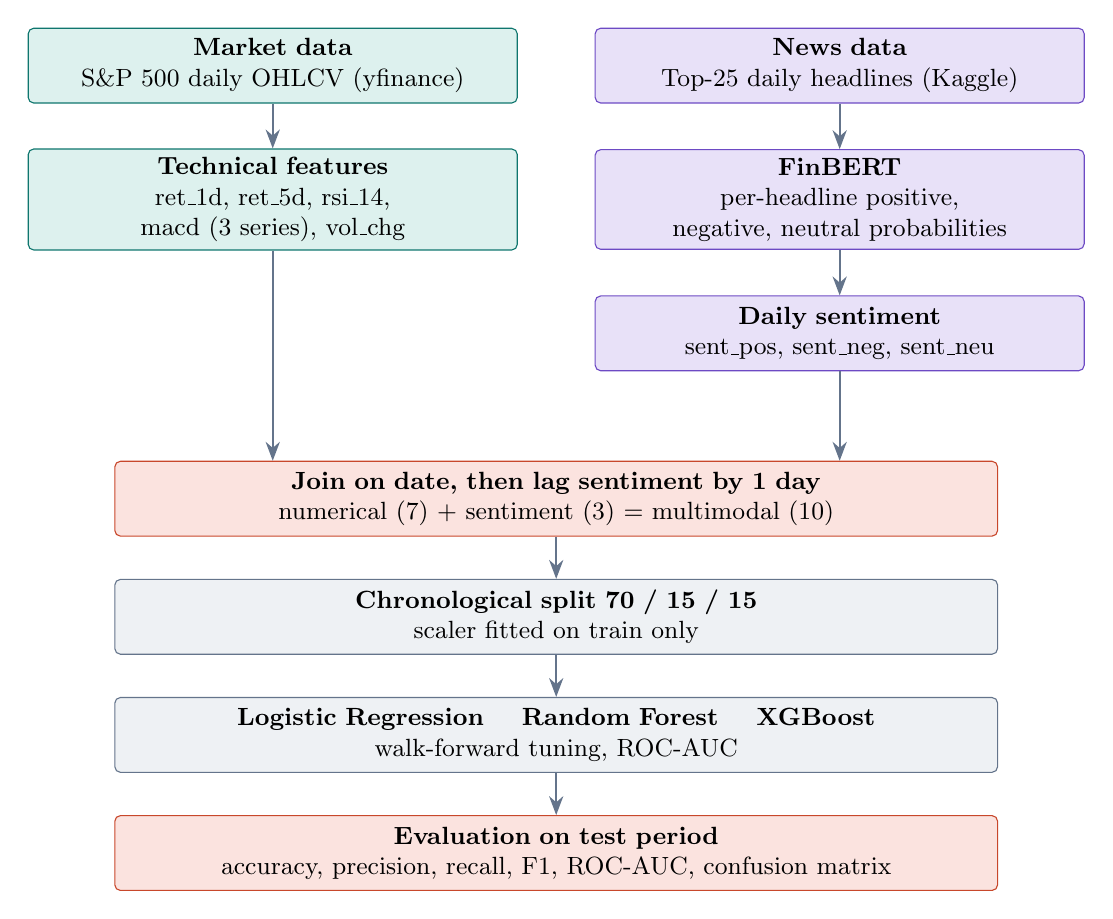
\begin{tikzpicture}
  \node[tbox] (mkt) at (-3.6,0) {\textbf{Market data}\\ S\&P 500 daily OHLCV (yfinance)};
  \node[tbox] (tech) at (-3.6,-1.7) {\textbf{Technical features}\\ ret\_1d, ret\_5d, rsi\_14,\\ macd (3 series), vol\_chg};
  \node[pbox] (news) at (3.6,0) {\textbf{News data}\\ Top-25 daily headlines (Kaggle)};
  \node[pbox] (fin) at (3.6,-1.7) {\textbf{FinBERT}\\ per-headline positive,\\ negative, neutral probabilities};
  \node[pbox] (agg) at (3.6,-3.4) {\textbf{Daily sentiment}\\ sent\_pos, sent\_neg, sent\_neu};
  \node[cbox, text width=11cm] (fuse) at (0,-5.5) {\textbf{Join on date, then lag sentiment by 1 day}\\ numerical (7) + sentiment (3) = multimodal (10)};
  \node[gbox, text width=11cm] (split) at (0,-7.0) {\textbf{Chronological split 70 / 15 / 15}\\ scaler fitted on train only};
  \node[gbox, text width=11cm] (models) at (0,-8.5) {\textbf{Logistic Regression \quad Random Forest \quad XGBoost}\\ walk-forward tuning, ROC-AUC};
  \node[cbox, text width=11cm] (eval) at (0,-10.0) {\textbf{Evaluation on test period}\\ accuracy, precision, recall, F1, ROC-AUC, confusion matrix};
  \draw[flow] (mkt) -- (tech);
  \draw[flow] (news) -- (fin);
  \draw[flow] (fin) -- (agg);
  \draw[flow] (tech.south) -- (tech.south |- fuse.north);
  \draw[flow] (agg.south) -- (agg.south |- fuse.north);
  \draw[flow] (fuse) -- (split);
  \draw[flow] (split) -- (models);
  \draw[flow] (models) -- (eval);
\end{tikzpicture}
\caption{Architecture of the proposed multimodal stock-direction prediction system.}
\label{fig:architecture}
\end{figure}

\section{Data Sources}

\subsection{Market data}
Daily S\&P 500 data (ticker \texttt{\textasciicircum GSPC}) are downloaded from Yahoo Finance~\cite{yahoofinance} with the \texttt{yfinance} library (unadjusted prices, \texttt{auto\_adjust=False}) for the period 1 August 2008 to 1 July 2016. The download contains the fields Open, High, Low, Close, Adj Close and Volume and is saved as \texttt{sp500\_raw.csv}; the closing value and the traded volume are used. Figure~\ref{fig:sp500} shows the closing value of the index over this period which the models divide chronologically into training, validation and test periods. The period includes the final phase of the financial crisis, the low point in March 2009, and the long recovery that followed.

\begin{figure}[!htbp]
\centering
\maybefigure{fig_sp500_split.png}{0.95\textwidth}{6cm}{Daily S\&P 500 closing value, August 2008 to July 2016, with the training, validation and test regions}
\caption{Daily S\&P 500 closing value from Yahoo Finance, August 2008 to July 2016. The first 70\% of trading days form the training set, the next 15\% the validation set and the final 15\% the test set.}
\label{fig:sp500}
\end{figure}

\subsection{News data}
The news modality comes from the Kaggle dataset ``Daily News for Stock Market Prediction''~\cite{kaggledaily}, file \texttt{Combined\_News\_DJIA.csv}. Each row corresponds to one date and contains the 25 most up-voted headlines (\texttt{Top1} to \texttt{Top25}) of the Reddit \texttt{r/worldnews} forum for that day. The file also contains a \texttt{Label} column describing the movement of the Dow Jones index; since our target is the S\&P 500 and the label is defined differently, this column is ignored.

\section{Numerical Branch}
For each trading day the branch computes the seven features of Chapter~3: \texttt{ret\_1d}, \texttt{ret\_5d}, \texttt{rsi\_14}, \texttt{macd}, \texttt{macd\_signal}, \texttt{macd\_hist} and \texttt{vol\_chg}. The target is created with Equation~\ref{eq:target}, by comparing the next day's close to the current close. The first rows, where rolling windows are incomplete (the RSI needs 14 days), and the last row, for which no next-day close exists, are removed; infinite volume changes are treated as missing. The result is saved as \texttt{features.csv}.

\section{Sentiment Branch}
The Kaggle file is restricted to the dates of the price data and converted from one column per headline (\texttt{Top1} to \texttt{Top25}) into one row per headline. Many headlines are stored as printed Python byte strings (\texttt{b'...'}); this wrapper, surrounding quotes and repeated white space are removed, headlines of five characters or fewer are dropped, and duplicate headlines within a day are removed. Every remaining headline (at most 25 per day, so close to 50,000 in total) is passed through the \texttt{ProsusAI/finbert} model, truncated to 64 tokens, in batches of 64. The model returns the three class probabilities for each headline. Scoring is the most expensive step of the project, so the headline-level scores are written to disk in chunks of 1,000 (\texttt{headline\_scores.csv}) and a rerun continues where it stopped. The scores are then averaged by date into three daily features, \texttt{sent\_pos}, \texttt{sent\_neg} and \texttt{sent\_neu}, together with the number of headlines of the day, and saved as \texttt{sentiment\_daily.csv}. A check confirms that the three probabilities of every headline sum to one.

\section{Fusion and Alignment}
The two tables (\texttt{features.csv} and \texttt{sentiment\_daily.csv}) are joined by an inner join on the calendar date, so that only days present in both are kept. This also removes weekends and holidays on which news exists but the market is closed.

The timing of information deserves care. The headlines dated $t$ describe events that occurred during day $t$. Whether a trader could have used them depends on when they appeared relative to the close, which the dataset does not record. To make sure that no sentiment that may have been published after the close is used, and to keep the design conservative, the project uses a lag of one trading day: the sentiment features aligned with day $t$ are those computed from the headlines of day $t-1$, and the model predicts the direction for day $t+1$ from technical features of day $t$ and sentiment of $t-1$. In the implementation, the \texttt{shift(1)} operation is applied \emph{after} the join, so that the shift moves along the sequence of trading days, not calendar days (a shift before the join would mis-align Mondays). The notebook verifies the lag with an assertion that each row holds the values its predecessor held before the shift, and the first row, which has no previous day, is dropped. Figure~\ref{fig:timeline} illustrates the alignment.

\begin{figure}[!htbp]
\centering
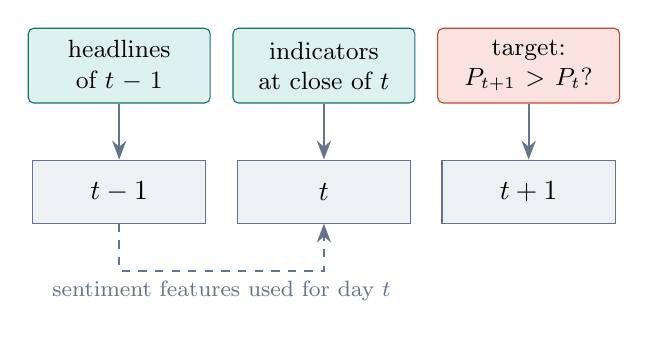
\begin{tikzpicture}[x=2.6cm, y=1cm]
  \foreach \i/\lab in {0/{$t-1$},1/{$t$},2/{$t+1$}} {
    \node[draw=grayline, fill=grayfill, minimum width=2.2cm, minimum height=0.8cm] (d\i) at (\i,0) {\lab};
  }
  \node[tbox, text width=2.1cm] (nh) at (0,1.6) {headlines of $t-1$};
  \node[tbox, text width=2.1cm] (ft) at (1,1.6) {indicators at close of $t$};
  \node[cbox, text width=2.1cm] (y) at (2,1.6) {target: $P_{t+1}>P_t$?};
  \draw[flow] (nh) -- (d0);
  \draw[flow] (ft) -- (d1);
  \draw[flow] (y) -- (d2);
  \draw[flow, dashed] (d0.south) -- ++(0,-0.6) -| node[pos=0.25, below, font=\footnotesize] {sentiment features used for day $t$} (d1.south);
\end{tikzpicture}
\caption{Temporal alignment. Features for day $t$ use technical indicators up to the close of $t$ and sentiment from headlines of $t-1$; the label is the direction of $P_{t+1}$ relative to $P_t$.}
\label{fig:timeline}
\end{figure}

\section{Feature Sets for the Ablation}
Three feature sets are defined, as in Table~\ref{tab:featuresets}. Every model is trained on every feature set, giving nine experiments. Comparing multimodal to numerical-only isolates the contribution of sentiment, and comparing multimodal to sentiment-only isolates the contribution of the technical indicators.

\begin{table}[!htbp]
\centering
\small
\begin{tabularx}{\textwidth}{@{}l c X@{}}
\toprule
Feature set & Size & Columns \\
\midrule
Numerical-only & 7 & ret\_1d, ret\_5d, rsi\_14, macd, macd\_signal, macd\_hist, vol\_chg \\
Sentiment-only & 3 & sent\_pos, sent\_neg, sent\_neu (lagged one day) \\
Multimodal & 10 & all of the above \\
\bottomrule
\end{tabularx}
\caption{Feature sets used in the ablation study.}
\label{tab:featuresets}
\end{table}

\section{Leakage-Control Design}
The following measures protect the evaluation from look-ahead bias.
\begin{enumerate}
  \item \textbf{Chronological split.} The first 70\% of days form the training set, the next 15\% the validation set, and the final 15\% the test set. No shuffling is performed.
  \item \textbf{Scaling.} A \texttt{StandardScaler} is fitted on the training set only, and applied unchanged to validation and test.
  \item \textbf{Sentiment lag.} Sentiment is shifted by one trading day after the join.
  \item \textbf{Walk-forward tuning.} Hyper-parameters are tuned with \texttt{TimeSeriesSplit} (three splits) on the training set, scored with ROC-AUC. The validation set is not used for selection; it only provides an additional ROC-AUC (\texttt{val\_auc}) for diagnosis, and the test set is not consulted during tuning.
  \item \textbf{Sanity checks.} In Step 2 an assertion confirms that no technical feature has an absolute correlation of 0.2 or more with the target (a value close to 1 would indicate a feature that contains the answer); in Step 4 assertions confirm the lag and that the training, validation and test periods follow one another in time without overlap.
  \item \textbf{Baseline.} The majority-class baseline is the accuracy obtained on the test set by always predicting the class that is more frequent in the training set; it is reported next to all models.
\end{enumerate}

\section{Models and Hyper-parameter Search}
Table~\ref{tab:grids} lists the search grids. They are intentionally small and conservative, because the number of training days (about 1,400) is small relative to the noise in the problem, and large grids would mostly increase the risk of overfitting the cross-validation folds. All stochastic components use the seed 42.

\begin{table}[!htbp]
\centering
\small
\begin{tabularx}{\textwidth}{@{}l X@{}}
\toprule
Model & Grid \\
\midrule
Logistic Regression & $C \in \{0.01, 0.1, 1, 10\}$ \\
Random Forest & 200 trees; max\_depth $\in \{3, 5, 8\}$; min\_samples\_leaf $\in \{5, 20\}$ \\
XGBoost & n\_estimators $\in \{100, 300\}$; max\_depth $\in \{2, 3, 4\}$; learning\_rate $\in \{0.03, 0.1\}$ \\
\bottomrule
\end{tabularx}
\caption{Hyper-parameter grids searched with walk-forward cross-validation.}
\label{tab:grids}
\end{table}

\section{Evaluation Protocol}
After tuning, each model is refitted on the whole training set with its best parameters (the default behaviour of \texttt{GridSearchCV}) and evaluated once on the test set. Class predictions use a probability threshold of 0.5, and the ROC curves and ROC-AUC use the predicted probabilities. The reported measures are accuracy, precision, recall, F1-score and ROC-AUC, together with confusion matrices. The ROC-AUC of the three feature sets is the main basis for the conclusion; accuracy is interpreted relative to the majority-class baseline and its margin of error.

\chapter{Implementation}

\section{Development Environment}
The project is implemented in Python as a sequence of Jupyter notebooks, one for each stage, so that every intermediate result can be inspected and saved to disk. The main libraries are \texttt{pandas} and \texttt{numpy} for data handling, \texttt{yfinance} for market data, \texttt{transformers} and \texttt{torch} for FinBERT, \texttt{tqdm} for progress bars, \texttt{scikit-learn}~\cite{pedregosa2011scikit} for preprocessing, Logistic Regression, Random Forest and evaluation, \texttt{xgboost}~\cite{chen2016xgboost} for gradient boosting, and \texttt{matplotlib} for figures. The work was carried out on a Windows machine using the Windows Subsystem for Linux and Visual Studio Code with the Jupyter extension. FinBERT runs on a GPU when one is available and on the CPU otherwise; the notebooks suggest running the scoring step on Google Colab with a GPU and copying the result back.

\section{Notebook Pipeline}
The pipeline consists of five notebooks, each reading the files written by the previous ones, followed by a sixth notebook that produces a demonstration forecast for the next trading day (Table~\ref{tab:notebooks}). The main settings are defined at the top of the relevant notebook: \texttt{LAG\_DAYS} and \texttt{TRAIN\_FRAC}/\texttt{VAL\_FRAC} in the fusion notebook, \texttt{RANDOM\_STATE} in the model notebook, and \texttt{SAMPLE} in the sentiment notebook (a switch for testing the scoring step on a few hundred headlines; it is \texttt{None} for the full run).

\begin{table}[!htbp]
\centering
\small
\begin{tabularx}{\textwidth}{@{}c p{3.4cm} X p{4.3cm}@{}}
\toprule
Step & Notebook & Purpose & Output \\
\midrule
1 & \texttt{yfinance} & Download S\&P 500 prices with yfinance, check missing values and duplicates & \texttt{sp500\_raw.csv} \\
2 & \texttt{features} & Technical features, target, leakage check & \texttt{features.csv} \\
3 & \texttt{sentiment} & Clean headlines, score with FinBERT, aggregate by day & \texttt{headline\_scores.csv}, \texttt{sentiment\_daily.csv} \\
4 & \texttt{fusion\_split} & Join, lag, chronological split & \texttt{fused.csv}, \texttt{train.csv}, \texttt{val.csv}, \texttt{test.csv} \\
5 & \texttt{models} & Tune, train, evaluate, ablate, demonstration forecast & \texttt{results.csv} \\
6 & \texttt{tomorrow} & Live next-day forecast from technical indicators only & printed forecast \\
\bottomrule
\end{tabularx}
\caption{The six notebooks of the project.}
\label{tab:notebooks}
\end{table}

\section{Step 1: Market Data}
The notebook first tests the download on a short period, then downloads the daily data for \texttt{\textasciicircum GSPC} from 1 August 2008 to 2 July 2016 (the end date is exclusive), flattens the column index that recent versions of \texttt{yfinance} return, removes the time zone from the dates and keeps the columns Date, Open, High, Low, Close, Adj Close and Volume. It prints the number of rows, the date range, missing values and duplicate dates, plots the closing value (Figure~\ref{fig:sp500}) and saves \texttt{data/sp500\_raw.csv}. Later steps read this file, so the prices are the same in every run, even if Yahoo Finance revises its data later.

\section{Step 2: Technical Features and Target}
The features are computed with vectorised \texttt{pandas} operations (Listing~\ref{lst:features}). The step ends with a leakage check: the correlation of each feature with the target is printed and an assertion stops the notebook if any absolute correlation is 0.2 or more.

\begin{lstlisting}[float=!htbp, caption={Technical features and target (Step 2).}, label={lst:features}]
def rsi(close, window=14):
    delta = close.diff()
    gain = delta.clip(lower=0)
    loss = -delta.clip(upper=0)
    avg_gain = gain.ewm(alpha=1 / window, adjust=False, min_periods=window).mean()
    avg_loss = loss.ewm(alpha=1 / window, adjust=False, min_periods=window).mean()
    rs = avg_gain / avg_loss
    return 100 - 100 / (1 + rs)

df = prices[["Date", "Close", "Volume"]].copy()
df["ret_1d"] = df["Close"].pct_change()
df["ret_5d"] = df["Close"].pct_change(5)
df["rsi_14"] = rsi(df["Close"])

ema12 = df["Close"].ewm(span=12, adjust=False).mean()
ema26 = df["Close"].ewm(span=26, adjust=False).mean()
macd = ema12 - ema26
macd_signal = macd.ewm(span=9, adjust=False).mean()
df["macd"] = macd / df["Close"] * 100      # scaled by price
df["macd_signal"] = macd_signal / df["Close"] * 100
df["macd_hist"] = df["macd"] - df["macd_signal"]
df["vol_chg"] = df["Volume"].pct_change().replace([np.inf, -np.inf], np.nan)

df["target"] = (df["Close"].shift(-1) > df["Close"]).astype(float)
df.loc[df.index[-1], "target"] = np.nan    # last day has no next-day close

TECH_COLS = ["ret_1d", "ret_5d", "rsi_14", "macd", "macd_signal",
             "macd_hist", "vol_chg"]
features = df.dropna(subset=TECH_COLS + ["target"]).reset_index(drop=True)
\end{lstlisting}

The notebook also prints the number of Down and Up days and the share of Up days, shows summary statistics and histograms of the features, and saves \texttt{data/features.csv}.

\section{Step 3: News Cleaning and Sentiment Scoring}
The Kaggle file is read, sorted by date and restricted to the dates of the price data. The 25 headline columns are converted into one row per headline with \texttt{melt}. Each headline is cleaned (the \texttt{b'...'} wrapper, quotes and repeated white space are removed), headlines of five characters or fewer are dropped, and duplicates within a day are removed. The headlines are then scored with the Hugging Face \texttt{pipeline} interface, requesting all class probabilities (\texttt{top\_k=None}), in chunks of 1,000 headlines whose results are appended to \texttt{data/headline\_scores.csv}, so that an interrupted run can resume (Listing~\ref{lst:finbert}).

\begin{lstlisting}[float=!htbp, caption={FinBERT scoring and daily aggregation (Step 3).}, label={lst:finbert}]
finbert = pipeline("text-classification", model="ProsusAI/finbert",
                   top_k=None, truncation=True, max_length=64,
                   device=0 if torch.cuda.is_available() else -1)

def score_headlines(texts, batch_size=64):
    out = finbert(list(texts), batch_size=batch_size)
    return pd.DataFrame([{d["label"].lower(): d["score"] for d in o}
                         for o in out])[["positive", "negative", "neutral"]]

CHUNK = 1000
for i in tqdm(range(0, len(remaining), CHUNK)):
    part = remaining.iloc[i:i + CHUNK].reset_index(drop=True)
    scored = pd.concat([part, score_headlines(part["headline"])], axis=1)
    done = pd.concat([done, scored], ignore_index=True)
    done.to_csv(SCORES_CSV, index=False)        # resumable cache

daily = (done.groupby("Date")
             .agg(sent_pos=("positive", "mean"),
                  sent_neg=("negative", "mean"),
                  sent_neu=("neutral", "mean"),
                  n_headlines=("positive", "size"))
             .reset_index())
daily.to_csv("data/sentiment_daily.csv", index=False)
\end{lstlisting}

The step also checks that the three scores of every headline sum to one, prints the share of headlines by their most probable label, lists the most positive and most negative headlines for a plausibility check, and plots a 30-day moving average of the daily sentiment.

\section{Step 4: Fusion, Lag and Split}
The fusion step performs the operations that most affect the validity of the study. Listing~\ref{lst:fusion} shows them in order. The notebook first reports how many trading days have no news and how many news days are not trading days (weekends and holidays, which the inner join drops).

\begin{lstlisting}[float=!htbp, caption={Alignment, lag and chronological split (Step 4).}, label={lst:fusion}]
TECH_COLS = ["ret_1d", "ret_5d", "rsi_14", "macd", "macd_signal",
             "macd_hist", "vol_chg"]
SENT_COLS = ["sent_pos", "sent_neg", "sent_neu"]

data = (features.merge(sentiment[["Date"] + SENT_COLS],
                       on="Date", how="inner")      # inner join on Date
                .sort_values("Date").reset_index(drop=True))

LAG_DAYS = 1
before = data[SENT_COLS].copy()
data[SENT_COLS] = data[SENT_COLS].shift(LAG_DAYS)   # lag AFTER the join
assert (data[SENT_COLS].iloc[LAG_DAYS:].values ==
        before.iloc[:-LAG_DAYS].values).all(), "Lag check failed"

data = data.dropna(subset=TECH_COLS + SENT_COLS + ["target"])
data = data.reset_index(drop=True)

FEATURE_SETS = {"numerical-only": TECH_COLS,
                "sentiment-only": SENT_COLS,
                "multimodal": TECH_COLS + SENT_COLS}

TRAIN_FRAC, VAL_FRAC = 0.70, 0.15
n = len(data)
i_train, i_val = int(n * TRAIN_FRAC), int(n * (TRAIN_FRAC + VAL_FRAC))
train, val, test = (data.iloc[:i_train].copy(),
                    data.iloc[i_train:i_val].copy(),
                    data.iloc[i_val:].copy())
assert train["Date"].max() < val["Date"].min() < val["Date"].max() < test["Date"].min()
\end{lstlisting}

The inner join keeps only days for which both modalities are present, the \texttt{shift} after the join implements the lag in trading days, and the assertion verifies it. The notebook then prints the size, date range and share of Up days of each part, computes the majority-class baseline from the training data, demonstrates that a \texttt{StandardScaler} fitted on the training rows gives approximately zero mean and unit variance on the training set but not exactly on the test set, plots the closing value coloured by split, and saves \texttt{fused.csv}, \texttt{train.csv}, \texttt{val.csv} and \texttt{test.csv}.

\section{Step 5: Training, Tuning and Evaluation}
Each of the three models is tuned for each of the three feature sets, using \texttt{GridSearchCV} with \texttt{TimeSeriesSplit(n\_splits=3)} and ROC-AUC as the scoring rule. A separate \texttt{StandardScaler} is fitted on the training rows of each feature set and applied to the validation and test rows. Listing~\ref{lst:train} shows the loop.

\begin{lstlisting}[float=!htbp, caption={Model tuning and test evaluation (Step 5).}, label={lst:train}]
MODELS = {
  "Logistic Regression": (LogisticRegression(max_iter=1000),
                          {"C": [0.01, 0.1, 1, 10]}),
  "Random Forest": (RandomForestClassifier(random_state=42, n_jobs=-1),
                    {"n_estimators": [200], "max_depth": [3, 5, 8],
                     "min_samples_leaf": [5, 20]}),
  "XGBoost": (XGBClassifier(eval_metric="logloss", random_state=42,
                            n_jobs=-1),
              {"n_estimators": [100, 300], "max_depth": [2, 3, 4],
               "learning_rate": [0.03, 0.1]}),
}

for fs_name, cols in FEATURE_SETS.items():
    scaler = StandardScaler().fit(train[cols])          # train only
    X_tr, X_val, X_te = (scaler.transform(p[cols])
                         for p in (train, val, test))
    for m_name, (est, grid) in MODELS.items():
        gs = GridSearchCV(est, grid, cv=TimeSeriesSplit(n_splits=3),
                          scoring="roc_auc", n_jobs=-1)
        gs.fit(X_tr, y_train)
        best = gs.best_estimator_
        proba = best.predict_proba(X_te)[:, 1]
        pred = (proba >= 0.5).astype(int)
        results.append({
            "feature_set": fs_name, "model": m_name,
            "cv_auc": gs.best_score_,
            "val_auc": roc_auc_score(y_val, best.predict_proba(X_val)[:, 1]),
            "accuracy": accuracy_score(y_test, pred),
            "precision": precision_score(y_test, pred, zero_division=0),
            "recall": recall_score(y_test, pred, zero_division=0),
            "f1": f1_score(y_test, pred, zero_division=0),
            "roc_auc": roc_auc_score(y_test, proba),
            "best_params": gs.best_params_})
\end{lstlisting}

The table of nine experiments is saved as \texttt{data/results.csv}. The notebook also computes the confusion matrices and ROC curves of all nine experiments, bar charts of test accuracy and ROC-AUC per feature set (with the chance line at 0.5 and the majority baseline), the feature importance of the three multimodal models (absolute coefficients for Logistic Regression, \texttt{feature\_importances\_} for the tree models), the multimodal minus numerical-only change per model, and the 95\% margin of error of the accuracy, $1.96\sqrt{p(1-p)/n}$ with $p$ the mean accuracy of the nine experiments and $n$ the number of test days.

Two further cells were added after the first results showed that most models predict Up on nearly every day. The first computes, for each of the nine fitted models, the share of test days predicted as Up and the balanced accuracy (the mean of the recall on Down days and the recall on Up days, for which 0.5 means no skill). The second produces a demonstration forecast: it selects the multimodal model with the highest \emph{validation} ROC-AUC (not the test AUC), refits it with its tuned parameters on the training and validation rows, and predicts the day after the last row of \texttt{fused.csv}. The data end on 30 June 2016, so the actual outcome is known and is printed for comparison.

\section{Step 6: Live Next-Day Forecast}
\label{sec:live}
The sixth notebook (\texttt{tomorrow.ipynb}) shows how the pipeline can be applied to current data. It downloads about 400 calendar days of S\&P 500 prices with \texttt{yfinance}, recomputes the seven technical features with the same function as Step 2, and asserts that this function reproduces \texttt{features.csv} exactly on the 2008 to 2016 prices, so that the live features are defined identically to the training features. A Logistic Regression with $C=0.01$ (the best numerical-only setting of Step 5) and a scaler are fitted on all rows of \texttt{fused.csv}, and the probability that the next trading day closes higher is computed from the most recent row. The notebook also prints the range of probabilities the model produced on the historical days, to show how far the current value is from indifference (0.5).

Only the numerical features are used. The Kaggle headline file ends in July 2016 and the project has no live headline source, so daily sentiment cannot be computed for the current date. Given that sentiment added no measurable value in Chapter~6, this restriction costs little, but it means that the forecast is made by a numerical-only model.

\section{Reproducibility}
All random seeds are fixed to 42 and every intermediate table is written to disk, so a stage can be rerun without repeating the earlier ones. In particular, the price download and the FinBERT scores are cached, which makes later runs independent of Yahoo Finance and avoids rescoring the headlines. The script \texttt{make\_results\_table.py} reads \texttt{results.csv} and produces the \LaTeX{} results table and the numerical macros used in the next chapter, so that the numbers in the report cannot drift from the numbers in the notebooks.

\section{Challenges Encountered}
The main practical difficulty was the installation of \texttt{transformers}: on an older Python 3.9 environment with an old NumPy, importing it failed with a \texttt{TypeError: 'type' object is not subscriptable}. Upgrading NumPy and restarting the kernel, pinning an older version of \texttt{transformers}, or creating a new environment with Python 3.11 resolved it. The other difficulty is the run time of the FinBERT step, which scores close to 50,000 headlines and is slow on a CPU; the resumable cache and the option of running the step on a GPU (for example on Google Colab) address this.

\chapter{Results and Discussion}

\section{Experimental Setup}
The experiments follow the protocol of Chapter~4. After the inner join and the one-day lag, the data are divided chronologically into a training set (the first 70\% of days: \TrainDays{} trading days, \TrainRange{}), a validation set (the next 15\%: \ValDays{} days, \ValRange{}) and a test set (the final 15\%: \TestDays{} days, \TestRange{}). The test set contains \UpShareTest{} Up days, so a classifier that always predicts the majority class reaches an accuracy of \BaselineAcc{}. With \TestDays{} test days, the 95\% margin of error on an accuracy near one half is \MarginErr{} percentage points. All numbers below come from the experiment notebooks (file \texttt{results.csv}) and are inserted into the report by the script \texttt{make\_results\_table.py}, so that the text and the tables cannot disagree.

\section{Main Results}
Table~\ref{tab:results} reports test-set performance of all nine experiments (three models on three feature sets).

\begin{table}[!htbp]
\centering
\small
\setlength{\tabcolsep}{4pt}
\begin{tabular}{@{}llccccc@{}}
\toprule
Feature set & Model & Accuracy & Precision & Recall & F1 & ROC-AUC \\
\midrule
Numerical-only & Logistic Regression & 0.498 & 0.500 & 0.993 & 0.665 & 0.520 \\
 & Random Forest & 0.512 & 0.507 & 0.913 & 0.652 & 0.487 \\
 & XGBoost & 0.498 & 0.500 & 0.926 & 0.649 & 0.482 \\
\midrule
Sentiment-only & Logistic Regression & 0.505 & 0.503 & 0.973 & 0.664 & 0.524 \\
 & Random Forest & 0.502 & 0.502 & 0.779 & 0.611 & 0.520 \\
 & XGBoost & 0.478 & 0.482 & 0.550 & 0.514 & 0.500 \\
\midrule
Multimodal & Logistic Regression & 0.498 & 0.500 & 0.933 & 0.651 & \textbf{0.539} \\
 & Random Forest & 0.512 & 0.507 & 0.966 & 0.665 & 0.483 \\
 & XGBoost & 0.522 & 0.515 & 0.826 & 0.634 & 0.481 \\
\midrule
\multicolumn{2}{l}{Majority-class baseline} & 0.502 & -- & -- & -- & 0.500 \\
\bottomrule
\end{tabular}

\caption{Test-set performance of each model on each feature set.}
\label{tab:results}
\end{table}

The best-performing combination by ROC-AUC is \BestModel{} on the \BestFeatureSet{} feature set, with a ROC-AUC of \BestAUC{} and an accuracy of \BestAcc{}. The majority-class baseline is \BaselineAcc{}.

\subsection{What the numbers show}
\begin{itemize}
  \item \textbf{Accuracy is at the baseline.} The nine accuracies range from 47.8\% (sentiment-only XGBoost) to 52.2\% (multimodal XGBoost). Every value is within the margin of error of the 50.2\% baseline, so none of the models is distinguishable from always guessing the majority class.
  \item \textbf{ROC-AUC is close to 0.5.} The values range from 0.481 to 0.539. The highest, multimodal Logistic Regression at \BestAUC{}, is only about 0.04 above chance, and at \TestDays{} test days the sampling uncertainty of an AUC is of the order of $\pm0.06$, so even this value cannot be separated from chance with confidence.
  \item \textbf{Sentiment adds little.} The best multimodal AUC (\MMBestAUC{}) exceeds the best numerical-only AUC (\NumBestAUC{}) by \AUCDelta{}, which is well inside the sampling uncertainty. For Random Forest and XGBoost the multimodal AUC is in fact slightly lower than that of the Logistic Regression models, and sentiment-only features alone reach at most 0.524.
  \item \textbf{High recall is an artefact.} Recall for the Up class is 0.55 to 0.99 for all models, while precision stays near 0.50. The models predict Up on most days, and recall is high because most of the Up days are caught by chance, not because of skill. The confusion matrices in Figure~\ref{fig:cm} confirm this: for numerical-only Logistic Regression, 296 of 297 predictions are Up. Table~\ref{tab:bias} shows that the balanced accuracy of all models is close to 0.5.
  \item \textbf{Validation is not a reliable guide.} The cross-validated AUC on the training data is about 0.47 to 0.52 for all experiments, and the validation AUC varies from 0.455 to 0.580 (the highest, numerical-only Logistic Regression, falls to 0.520 on the test set). This instability is typical of a signal that is too weak to be measured reliably.
\end{itemize}

\section{Effect of the Feature Set}
The ablation compares the best ROC-AUC obtained with numerical features alone (\NumBestAUC) to the best obtained with the multimodal features (\MMBestAUC), a difference of \AUCDelta{}. Figure~\ref{fig:roc} shows the ROC curves of the three models for each feature set, and Figure~\ref{fig:featimp} shows which features the tree-based models rely on.

\begin{figure}[!htbp]
\centering
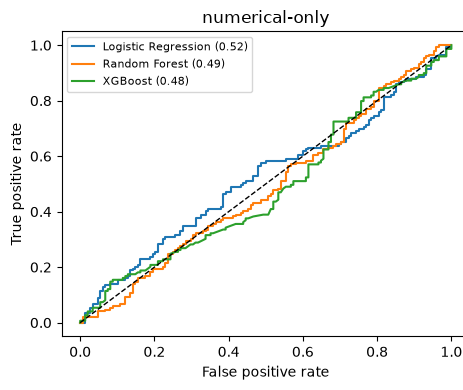
\includegraphics[width=0.49\textwidth]{figures/fig_roc_numerical.png}\hfill
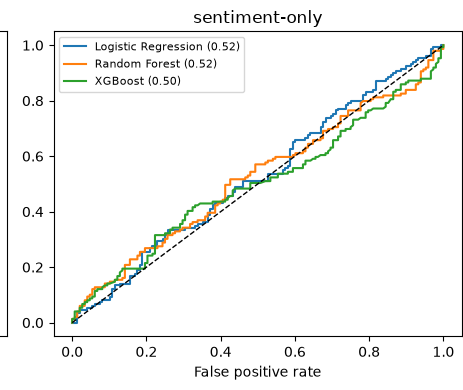
\includegraphics[width=0.49\textwidth]{figures/fig_roc_sentiment.png}\\[4pt]
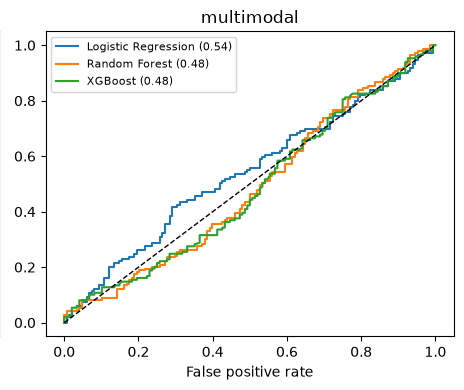
\includegraphics[width=0.49\textwidth]{figures/fig_roc_multimodal.png}
\caption{ROC curves on the test set for the three feature sets; the legend gives the ROC-AUC of each model and the dashed line is chance.}
\label{fig:roc}
\end{figure}

\begin{figure}[!htbp]
\centering
\maybefigure{fig_feature_importance.png}{0.98\textwidth}{6.5cm}{Feature importance of the multimodal Random Forest or XGBoost model, with sentiment features highlighted}
\caption{Feature importance in the multimodal models: absolute coefficient for Logistic Regression and impurity-based importance for Random Forest and XGBoost (\texttt{sent\_pos}, \texttt{sent\_neg}, \texttt{sent\_neu} correspond to the three daily sentiment means).}
\label{fig:featimp}
\end{figure}

\section{Confusion Matrices}
Accuracy alone does not reveal whether a model simply predicts one class most of the time. Figure~\ref{fig:cm} shows the confusion matrices of all nine experiments. Nearly all models predict Up on most days, so recall for Up is high and almost no Down day is identified correctly; the matrices make this visible.

\begin{figure}[!htbp]
\centering
\maybefigure{fig_confusion.png}{0.95\textwidth}{5.5cm}{Three confusion matrices side by side (numerical-only, sentiment-only, multimodal) for the best model of each set}
\caption{Confusion matrices of all nine experiments on the test set (rows: true class, columns: predicted class).}
\label{fig:cm}
\end{figure}

\section{Bias Towards the Up Class}
The high recall and F1-score of most models (Table~\ref{tab:results}) invite a misreading, so the share of Up predictions and the balanced accuracy were computed for every experiment (Table~\ref{tab:bias}). Balanced accuracy is the mean of the recall on Down days and the recall on Up days; a model without skill obtains 0.5 whatever its class bias. The test set contains 50.2\% Up days.

\begin{table}[!htbp]
\centering
\small
\begin{tabular}{@{}llccc@{}}
\toprule
Feature set & Model & Predicted Up & Accuracy & Balanced accuracy \\
\midrule
Numerical-only & Logistic Regression & 0.997 & 0.498 & 0.497 \\
 & Random Forest & 0.902 & 0.512 & 0.510 \\
 & XGBoost & 0.929 & 0.498 & 0.497 \\
\midrule
Sentiment-only & Logistic Regression & 0.970 & 0.505 & 0.503 \\
 & Random Forest & 0.778 & 0.502 & 0.501 \\
 & XGBoost & 0.572 & 0.478 & 0.478 \\
\midrule
Multimodal & Logistic Regression & 0.936 & 0.498 & 0.497 \\
 & Random Forest & 0.956 & 0.512 & 0.510 \\
 & XGBoost & 0.805 & 0.522 & 0.521 \\
\bottomrule
\end{tabular}
\caption{Share of test days predicted as Up, accuracy and balanced accuracy of the nine experiments.}
\label{tab:bias}
\end{table}

Eight of the nine models predict Up on more than three quarters of the days, and numerical-only Logistic Regression does so on 99.7\% of them. Their balanced accuracy lies between 0.478 and 0.521, that is, at the no-skill value of 0.5 within the sampling error. The F1-scores of about 0.65 are therefore a consequence of the Up bias and not evidence of skill: a classifier that always predicts Up has recall 1.0 and an F1-score of 0.67 on this test set.

\section{Demonstration Forecasts}
\label{sec:forecast}
Two forecasts were produced to show how the trained pipeline is used. They are demonstrations of the procedure, not evidence of skill: a single call is right with probability one half even for a coin flip.

\paragraph{Last day of the data set.} The multimodal model with the highest validation ROC-AUC is Logistic Regression ($C=0.01$, validation AUC 0.538). Refitted on the training and validation rows, it gives a probability of 0.517 that the market closes higher after 30 June 2016, that is, the prediction Up. The actual direction was Up. The probability is very close to 0.5, so the model expresses almost no confidence.

\paragraph{Current data.} The notebook \texttt{tomorrow.ipynb} downloads recent S\&P 500 prices and applies the numerical-only Logistic Regression ($C=0.01$), fitted on all 1,978 days of 2008 to 2016 (Section~\ref{sec:live}). The most recent close in the data downloaded was 7,561.67 on 13 November 2026, and the model gave a probability of 0.561 that the next trading day closes higher, that is, Up. For reference, the probabilities produced by the same model on the historical days range from 0.348 to 0.686 with a median of 0.540, so 0.561 is a weak, near-neutral signal. Because the model has no measured skill on the test period (Table~\ref{tab:bias}), this output must not be used as a trading signal. Sentiment is not part of this forecast because no current headline feed is available.

\section{How to Interpret the Results}
\label{sec:interpret}
The following reading guide applies regardless of the specific numbers obtained.
\begin{itemize}
  \item \textbf{Compare with the baseline first.} An accuracy equal to the majority-class share indicates that the model has learned nothing beyond the class balance. Only accuracy above baseline by more than the margin of error is evidence of skill.
  \item \textbf{Use ROC-AUC for ranking skill.} A ROC-AUC near 0.50 means the model's scores do not rank Up days above Down days. Values in the low 0.50s are typical for this task and are at the edge of what can be distinguished from noise on a test set of a few hundred days.
  \item \textbf{Judge the multimodal benefit by the difference.} If multimodal and numerical-only ROC-AUC differ by less than the sampling uncertainty, the honest conclusion is that sentiment did not demonstrably help; if multimodal is clearly higher, sentiment contributes complementary information.
  \item \textbf{Be suspicious of very high scores.} Next-day direction is close to unpredictable. Accuracy near 90\% or above would indicate leakage, as in the 100\% figure of the reviewed preprint, and would call for a check of the pipeline, not a celebration.
\end{itemize}

\section{Discussion}
\subsection{Why the signal is expected to be weak}
Several features of the problem limit what any model can achieve. The efficient market hypothesis predicts that public information is rapidly incorporated into prices. Daily index direction is the net effect of thousands of simultaneous events, and most of its variance is unrelated to the average sentiment of 25 headlines from a general world-news forum. The Reddit headlines are not specific to finance: many concern politics and conflicts, and FinBERT, trained on financial text, may assign confident sentiment to sentences outside its domain.

\subsection{Role of each model}
Logistic Regression has little capacity to overfit, so it is expected to be competitive with the more flexible models when the signal is weak. Random Forest and XGBoost can capture interactions but also fit noise; their depth limits and the walk-forward tuning are intended to restrain them. If the flexible models achieve a higher cross-validated AUC but not a higher test AUC, that is a sign of overfitting to the validation folds.

\subsection{Effect of the sentiment lag}
The one-day lag makes the design conservative. It guarantees that the sentiment used on day $t$ was available before the target day, but it may also discard a genuine same-day relationship, because headlines published in the morning could influence the same day's close. This design choice favours validity over apparent performance, and the lag can be set to zero as a sensitivity check (with the caveat that the result then depends on the unknown publication time).

\subsection{Limitations}
\begin{itemize}
  \item The test period is a single contiguous stretch of a rising market, so the results may not generalise to other regimes such as sharp declines.
  \item The text input is limited to Reddit headlines, which are crowd-curated and not guaranteed to be representative of financial news flow.
  \item The sentiment encoder is applied to headlines without fine-tuning on the target task.
  \item The study evaluates classification quality and not trading performance, so transaction costs and risk are not considered.
  \item With a few hundred test days, differences of a few percentage points are within sampling error.
\end{itemize}

\chapter{Conclusion and Future Work}

\section{Conclusion}
This project designed and implemented a multimodal machine learning framework for predicting the next-day direction of the S\&P 500 index. Technical features derived from market data (returns, RSI, MACD and volume change) were combined by early fusion with daily sentiment scores obtained by applying FinBERT to news headlines. Logistic Regression, Random Forest and XGBoost were trained on three feature sets, namely numerical-only, sentiment-only and multimodal, and evaluated with accuracy, precision, recall, F1-score, ROC-AUC and confusion matrices.

The main contribution is the evaluation design. The review of recent work in Chapter~2 showed that results in this area are often reported with accuracy only, without baselines, or with splits that allow look-ahead leakage. In response, the framework uses a strictly chronological 70/15/15 split, a one-day lag of the sentiment features applied after the join, scaling fitted on training data only, walk-forward hyper-parameter tuning and a majority-class baseline with a stated margin of error. The ablation across feature sets isolates the effect of each modality, so the conclusion on whether sentiment adds value does not rest on a single number.

The test-set results (Chapter~6) show that none of the nine model and feature-set combinations demonstrated predictive skill. Accuracies lie between 47.8\% and 52.2\% against a majority-class baseline of \BaselineAcc{}, and ROC-AUC lies between 0.481 and \BestAUC{}, the latter reached by \BestModel{} on the \BestFeatureSet{} features. The multimodal model improved on the best numerical-only ROC-AUC by only \AUCDelta{}, which is within sampling error for \TestDays{} test days. Most models also fell back to predicting the Up class for the great majority of days: eight of the nine predicted Up on more than three quarters of the test days, and their balanced accuracy was between 0.478 and 0.521, that is, at the no-skill value of 0.5.

We therefore conclude that, in this experiment, combining FinBERT sentiment of Reddit world-news headlines with technical indicators did not produce a measurable improvement in next-day direction prediction of the S\&P 500. This is a legitimate finding: it is consistent with the efficient market hypothesis and with the modest accuracies (about 57\% at best) reported by comparable headline-based studies, and it contrasts with the near-perfect scores of leakage-prone designs. The value of the project lies in the evaluation design, which makes this negative result trustworthy rather than in a claim of predictive power.

The pipeline was also applied to current data in a demonstration (Section~\ref{sec:forecast}). Using only technical indicators, because no live headline source was available, the numerical-only Logistic Regression gave a probability of 0.561 that the next trading day after 13 November 2026 closes higher. This shows that the framework can produce a forecast for the coming day, but given the test results it should be read as a demonstration of the procedure, not as a signal.

\section{Future Work}
Several extensions are natural.
\begin{enumerate}
  \item \textbf{Live news.} Replace the historical corpus with a live headline feed, so that the multimodal model, and not only the numerical-only model of the demonstration, can produce a prediction for the coming trading day. This requires a news source with a known publication time, daily FinBERT scoring, and a decision on the cut-off time relative to the market close.
  \item \textbf{Richer text.} Use finance-specific sources (newswires, earnings calls, filings) and full articles rather than headlines, and weight headlines by relevance or source reliability.
  \item \textbf{Fine-tuning.} Fine-tune the language model on the prediction target, or use embeddings from the model rather than three probabilities, at the cost of a larger and riskier model.
  \item \textbf{Sequence models.} Use LSTM or GRU networks that consume a window of past days, and late or intermediate fusion architectures.
  \item \textbf{More robust evaluation.} Use rolling-origin evaluation over several test windows and several market regimes, add statistical tests for the difference between models, and extend the study to other indices and to longer horizons.
  \item \textbf{Economic evaluation.} Translate predictions into a simple trading rule and report returns after transaction costs and risk-adjusted measures, to move from classification quality to practical value.
  \item \textbf{Explainability.} Apply Shapley-value analysis to quantify the contribution of each modality to individual predictions.
\end{enumerate}


% References
\renewcommand{\bibname}{References}
\addcontentsline{toc}{chapter}{\bibname}
\bibliographystyle{plain}
\bibliography{references}

% Appendices
\appendix
\chapter{Supplementary Material}

\section{Software Environment}
Table~\ref{tab:env} lists the software used. The notebooks were run with Python 3.13 and 3.14 (the saved outputs show 3.14 on the development machine); the exact package versions can be recorded with \texttt{pip freeze}.

\begin{table}[!htbp]
\centering
\small
\begin{tabular}{@{}lp{7.5cm}@{}}
\toprule
Component & Purpose \\
\midrule
Python 3.13 or later & Language \\
pandas, numpy & Data handling \\
yfinance & S\&P 500 daily data download \\
transformers, torch, tqdm & FinBERT (\texttt{ProsusAI/finbert}) and progress bars \\
scikit-learn & Scaling, Logistic Regression, Random Forest, metrics, \texttt{TimeSeriesSplit} \\
xgboost & Gradient-boosted trees \\
matplotlib & Figures \\
JupyterLab or VS Code with Jupyter & Notebook environment \\
\bottomrule
\end{tabular}
\caption{Software used in the project.}
\label{tab:env}
\end{table}

\section{Project File Layout}
\begin{lstlisting}[float=!htbp, language={}, caption={Layout of the project directory.}]
Stock_Prediction/
  yfinance.ipynb      features.ipynb      sentiment.ipynb
  fusion_split.ipynb  models.ipynb        tomorrow.ipynb
  README.md           PRESENTATION.md
  data/
    Combined_News_DJIA.csv      (Kaggle)
    sp500_raw.csv     features.csv
    headline_scores.csv  sentiment_daily.csv
    fused.csv  train.csv  val.csv  test.csv
    results.csv
  report/                       (this LaTeX project)
    main.tex  chapters/  figures/  tables/  data/
\end{lstlisting}

\section{Computing the Numbers in the Report}
After the notebooks have been run on the real data, the report numbers are generated with the script below. It reads \texttt{results.csv} and, because \texttt{train.csv}, \texttt{val.csv} and \texttt{test.csv} are present in the same folder (\texttt{report/data/}), the split files, from which it takes the number of days and the date ranges of the three parts; it writes the results table and the numerical macros, and the report is then recompiled. If the split files are absent, the number of test days and of Up days can be passed as arguments instead. The balanced-accuracy table (Table~\ref{tab:bias}) and the two demonstration forecasts (Section~\ref{sec:forecast}) are copied from the printed output of the notebooks \texttt{models.ipynb} and \texttt{tomorrow.ipynb} and must be updated by hand if those notebooks are rerun.

\begin{lstlisting}[float=!htbp, caption={Command sequence to update the report with real results.}]
python make_results_table.py data/ tables/
pdflatex main && bibtex main && pdflatex main && pdflatex main
\end{lstlisting}

\section{Individual Contributions}
Table~\ref{tab:team} lists the team members and their responsibilities in the project.

\begin{table}[!htbp]
\centering
\small
\begin{tabularx}{\textwidth}{@{}l l X@{}}
\toprule
Member & Roll & Main responsibility \\
\midrule
Kundan Kumar & 6 & Model training, evaluation and results \\
Soham Mohanty & 3 & Market data and technical features \\
Priyanshu Sekhar Badhei & 4 & News data and FinBERT sentiment \\
Naman Verma & 2 & Fusion, alignment and leakage checks \\
Tejash Arya & 15 & Documentation, literature review and presentation \\
\bottomrule
\end{tabularx}
\caption{Team members and responsibilities (to be adjusted to the final division of work).}
\label{tab:team}
\end{table}


\end{document}
